\section{Dateisysteme EXT2 und EXT4}
\textbf{Partition: }Teil eines Datenträgers, wird selbst wie ein Datenträger behandelt
\textbf{Volume: }Datenträger oder Partition
\textbf{Sektor: }kleinste logische Untereinheit eines Volumens, Daten als Sektoren transferiert, Grösse durch HW bestimmt, enthält Header, Daten und Error-Correction-Codes
\textbf{Format: }Lyout der logischen Strukturen, vom Dateisystem definiert

\subsubsection{Block/Inodes}
Blockgrösse: 1 KB, 2KB oder 4KB (Standard)\\
Block enthält nur Daten einer einzigen Datei\\
%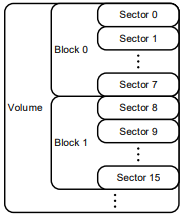
\includegraphics[scale = 0.40]{grafiken/block.PNG}
%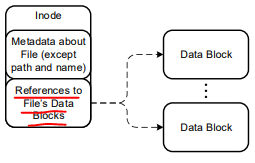
\includegraphics[scale = 0.40]{grafiken/inode.PNG}
%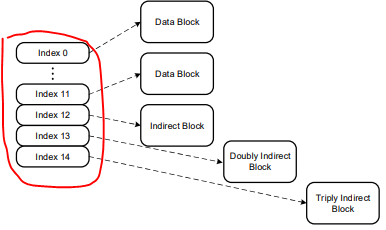
\includegraphics[scale = 0.40]{grafiken/inodes_referenzen.PNG}
Inodes-Grösse: fixe Grösse pro Volume, 2er-Potenz, mind. 128 Byte, max. 1 Block

\subsubsection{Anzahl referenzierter Blöcke}
Blockliste (60 Byte): 15 Blocknr. à 32 Bit\\
Anzahl abhängig von der Blockgrösse:\\
Index 0-12 \textbf{Indirekter Block:} Blockgr. in Bits/32 Bit\\
Index 13 \textbf{Doppelt indir. Block:} (Blockgr. in Bits/32 Bit)$^{2}$\\
Index 14 \textbf{Dreifach indir. Block:} (Blockgr. in Bits/32 Bit)$^3$

%\subsubsection{File-Holes}
%Bereiche in der Datei, in der nur Nullen stehen.\\
%Wenn Index = 0, ist ganzer Block mit Nullen gefüllt.

\subsection{Verzeichnisse}
Inode, dessen Datenbereich Entries enthält\\
automatisch angelegte Entries:
\prgc{.} | eigener Inode gespeichert, \prgc{..} | Inode des Elternverzeichnisses\\
%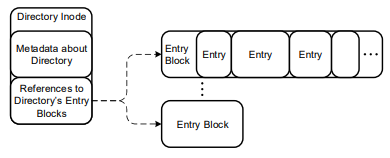
\includegraphics[scale = 0.3]{grafiken/verzeichnis.PNG}\\
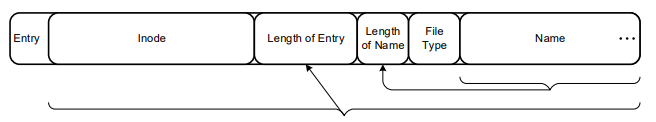
\includegraphics[scale = 0.4]{grafiken/entry.PNG}

\subsubsection{Entries}
Länge variabel 8 - 263 Bytes, Vielfaches von 4 Bytes\\
4 Bytes Inode, 2 Byte Length of Entry, 1 Byte Length of Name, 1 Byte File Type (1=Datei, 2=Verzeichnis, 7=Symbolischer Link), 0-255 Byte Name (Ascii) 

\subsection{Links}
\textbf{Hardlink: }Inode ist gleich, Pfade sind verschieden
\textbf{Symbolischer Link: }wie Datei, die Pfad auf andere Datei enthält, (Pfad < 60 Zeichen: Pfad direkt in Array gespeichert, ohne Blockallokation, sonst Bockallokation)

\subsection{Blockgruppe}
Volume wird in Blockgruppen unterteilt\\
Gruppengrösse bis zu \textcolor{blue}{Faktor 8} der Anzahl Bytes pro Block\\
z.B. Blockgrösse 4 KB $\rightarrow$ Gruppegrösse: 32k Blöcke
Anzahl Blöcke pro Gruppe für alle Gruppen gleich\\
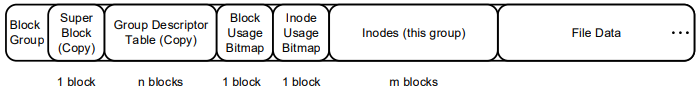
\includegraphics[scale = 0.4]{grafiken/blockgruppe.PNG}

\subsubsection{Superblock}
enthält alle Meta-Daten übers Volume (Anzahlen, Bytes pro Block etc., verschiedene Zeitpunkte, verschiedene Statusbytes, erster Inode, Feature-Flags)\\
startet immer an Byte 1024 (evtl. Boot-Daten davor)

\subsubsection{Gruppendeskriptor}
32 Bytes, Beschreibung einer Blockgruppe (Blocknummern Bitmaps/Inode-Tabelle, Anzahl freier Inodes/Blöcke, Anzahl Verzeichnisse pro Gruppe)

\subsubsection{Sparse Superblocks}
Die Kopien des Superblocks \& Group Descriptor Table werden nur noch in Blockgruppe 0 \& 1, sowie in allen reinen Potenzen von 3/5/7 gehalten

\subsubsection{Lokalisierung eines Inodes}
Alle Inodes gelten als eine grosse Tabelle\\
Inode-Nr. beginnen bei 1\\
Blockgruppe = (Inode - 1)/Anz. Inodes pro Gruppe\\
Index des Inodes in Gruppe = (Inode - 1) \% Anz. Inodes pro Gruppe\\
Sektor und Offset anhand Superblock

%\subsubsection{Erzeugen von Inodes}
%Neue Verzeichnisse in Blockgruppen, die überdurchschnittlich viele freie Blöcke haben\\
%Dateien möglichst in Blockgruppe des Verzeichnisses oder in nahe Gruppe

\subsection{Ext4}
Inodes 256 Bytes statt 128, Gruppendeskrip. 64 Bytes statt 32, Blockgrösse bis 64 KB
%Extent Trees (Assoziation von Blöcken zu Inodes), Journaling

\subsubsection{Extent Trees}
Tree (60 Byte): 5 Elemente à 12 Byte, max. Tiefe 5
+ Grosse Dateien, Nur 1 Extent Speicher vs. Jede Blocknr.
%Header: Anzahl nachfolgender Elemente auf gleichem Level, Level-Angabe\\
%Index (innerer Knoten): Index-Eintrag (12 Bytes), Index-Block\\
%Index-Eintrag: enthält Nummer des physischen Index-Blocks, kleinste logische Blocknummer aller Kindknoten\\
%Index-Block: eigener Tree-Header, Referenzen auf Kind-Knoten
%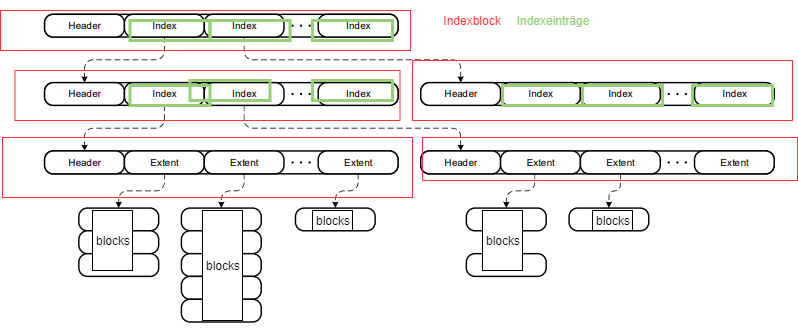
\includegraphics[scale = 0.3]{grafiken/extent_tree (1).png}

\subsection{Journaling}
\textbf{Ablauf bei Dateierweiterung:} Allokation neuer Blöcke, Anpass. Inode, Anpassung Block-Usage-Bitmap/Counter freier Blöcke, Schreiben von Daten in Datei\\
\textbf{System ohne Journaling:} Muss alle Meta-Daten überprüfen
\textbf{mit Journaling:} nur Metadaten, vom Journal

%\subsubsection{Ablauf}
%1. Daten als Tranksaktionen ins Journal (reservierte Datei vor allen Daten) $\rightarrow$ sehr schnell, da nacheinander folgende Blöcke beschrieben
%2. An endgültige Position geschrieben (Committing)
%3. Daten nach Commit aus Transaktion entfernt\\
\textbf{Journal Replay:} Bei Systemneustart, Untersuch der Metadaten auf korrupte Werte anhand Journal
\textbf{Journal: }Metadaten \& Dateiinhalte ins Journal \textcolor{green}{+} maximale Datensicherheit, \textcolor{red}{-} Geschwindigkeit
\textbf{Ordered: }1. Metadaten ins Journal 2. File Content direkt an finale Position 3. Commit \textcolor{green}{+} Dateien nach Commit richtigen Inhalt \textcolor{red}{-} geringere Geschwindigkeit
\textbf{Writeback: }dito Ordered aber Commit \& Schreiben der Daten in beliebiger Reihenfolge \textcolor{green}{+}sehr schnell \textcolor{red}{-}Dateien evtl. Datenmüll
